\documentclass[11pt,a4paper]{article}

% Encodage et langue francaise
\usepackage[T1]{fontenc}
\usepackage[utf8]{inputenc}
\usepackage[french]{babel}
\usepackage{lmodern}
\usepackage[margin=2cm]{geometry}
\usepackage{amsmath,amssymb}
\usepackage{graphicx}
\usepackage{float}
\usepackage{booktabs}
\usepackage{xcolor}
\usepackage{hyperref}
\usepackage{enumitem}

% Dossiers ou Overleaf cherche les images
\graphicspath{{assets/}{./assets/}{./}}

\definecolor{primary}{RGB}{25, 55, 100}
\definecolor{accent}{RGB}{40, 120, 80}

\hypersetup{
    colorlinks=true,
    linkcolor=primary,
    urlcolor=primary,
    pdftitle={Rapport de Projet - Secure GPU Upscaler},
    pdfauthor={Mohamed B.}
}

\begin{document}

% EN-TETE PERSONNEL / PROFIL ETUDIANT
\begin{center}
    {\LARGE\bfseries\color{primary} Projet Personnel : Secure GPU Upscaler}\\[0.2cm]
    {\large\textbf{Super-Résolution d'Images sur GPU NVIDIA, Optimisation FP16 et Sécurité Anti-DoS}}\\[0.25cm]
    \textbf{Mohamed B.} -- Étudiant en école d'ingénieurs (1\iere{} année)\\[0.1cm]
    Passionné par le matériel NVIDIA, l'optimisation GPU, le DevOps et la cybersécurité\\[0.1cm]
    \textbf{Dépôt GitHub du projet :} \url{https://github.com/Git-MohamedB/secure-gpu-upscaler}
\end{center}

\vspace{0.2cm}
\hrule
\vspace{0.4cm}

% 1. MOTIVATION PERSONNELLE
\section{Pourquoi j'ai réalisé ce projet ? (Ma motivation)}

Depuis toujours, je suis passionné par le matériel informatique et les technologies graphiques NVIDIA (l'architecture des GPU, les Tensor Cores, le DLSS dans les jeux vidéo). Je voulais comprendre comment fonctionne réellement l'upscaling par intelligence artificielle sous le capot, au lieu de simplement l'utiliser comme une boîte noire.

Dans le même temps, je voulais développer des compétences solides en \textbf{DevOps} et en \textbf{cybersécurité applicative}. Lancer un modèle de Deep Learning dans un notebook Jupyter sur son propre PC est facile. Mais créer un \textbf{vrai microservice prêt pour la production}, qui ne crashe pas dès qu'une image est trop grande et qui résiste aux attaques malveillantes, c'est un vrai défi d'ingénierie.

J'ai donc conçu ce projet pour relier ces centres d'intérêt :
\begin{itemize}[noitemsep]
    \item Exploiter ma carte graphique (\textbf{NVIDIA GeForce RTX 4060 Ti}) avec PyTorch et CUDA ;
    \item Résoudre mathématiquement le problème de saturation mémoire grâce au tuilage (\textit{tiling}) ;
    \item Mettre en place une API moderne avec FastAPI ;
    \item Sécuriser et conteneuriser le service avec Docker selon les bonnes pratiques de sécurité.
\end{itemize}

% 2. CE QUE J'AI APPRIS CONCRETEMENT
\section{Ce que ce projet m'a appris concrètement}

Ce projet m'a permis de sortir de la théorie et d'apprendre énormément sur le terrain :

\begin{enumerate}[leftmargin=*]
    \item \textbf{La gestion de la mémoire GPU (VRAM) et le format FP16 :}
    J'ai appris comment les données sont stockées en mémoire vidéo. En passant le modèle de la simple précision (FP32, 4 octets par valeur) à la demi-précision (\textbf{FP16}, 2 octets), j'ai divisé par deux l'empreinte mémoire des tenseurs et accéléré les calculs grâce aux cœurs Tensor de ma carte.
    
    \item \textbf{Résoudre les crashs par Tuilage (\textit{Tiling}) :}
    Au début, quand j'essayais d'agrandir une image de haute résolution, mon GPU affichait immédiatement l'erreur redoutée \texttt{CUDA OutOfMemoryError}. J'ai implémenté un algorithme qui découpe l'image en tuiles de $512 \times 512$ pixels avec une petite marge de sécurité (10 pixels de recouvrement pour éviter les démarcations visibles). Grâce à ça, la mémoire vidéo utilisée reste plafonnée à \textbf{560 Mo}, peu importe que l'image soit petite ou énorme.
    
    \item \textbf{Évaluer la qualité avec des formules scientifiques réelles :}
    J'ai découvert qu'on ne juge pas une amélioration d'image au hasard. J'ai implémenté le calcul du \textbf{PSNR} (fidélité pixel par pixel) et du \textbf{SSIM} (qui mesure si l'œil humain perçoit bien les textures, les contrastes et les contours).
    
    \item \textbf{La cybersécurité applicative (défense contre les DoS) :}
    J'ai appris qu'une API publique d'IA est très vulnérable. J'ai codé des filtres stricts :
    \begin{itemize}[noitemsep]
        \item Rejet immédiat si le fichier dépasse 10 Mo (évite de remplir la RAM) ;
        \item Vérification des \textit{Magic Bytes} (signatures binaires des fichiers) pour bloquer les faux fichiers texte renommés en \texttt{.png} ;
        \item Protection contre les bombes de décompression : je lis les dimensions dans l'en-tête de l'image sans décompresser les pixels, et je bloque au-delà de $2048 \times 2048$.
    \end{itemize}

    \item \textbf{Le durcissement conteneur (DevSecOps) :}
    J'ai appris à configurer Docker proprement : ne jamais lancer le conteneur en utilisateur \texttt{root} (création d'un utilisateur dédié \texttt{appuser}), interdire l'élévation de privilèges (\texttt{no-new-privileges:true}), et limiter les ressources via les quotas Linux cgroups (4 Go de RAM et 2 CPU maximum).
\end{enumerate}

% 3. LES MATHS EXPLIQUEES SIMPLEMENT
\section{Les formules mathématiques : d'où elles viennent et à quoi elles servent}

Dans le projet, les choix techniques et l'évaluation reposent sur 4 formules standards :

\subsection{1. Taille d'un tenseur en mémoire GPU (Norme IEEE 754)}
L'espace mémoire occupé par une image en mémoire vidéo est calculé par la formule :
\begin{equation}
    \text{Taille} = H \times W \times C \times S_{\text{dtype}}
\end{equation}
où $H$ est la hauteur, $W$ la largeur, $C=3$ les canaux (Rouge, Vert, Bleu), et $S_{\text{dtype}}$ la taille du type de données définie par la norme internationale \textbf{IEEE 754} :
\begin{itemize}[noitemsep]
    \item En FP32 (standard) : 4 octets par valeur.
    \item En FP16 (demi-précision) : 2 octets par valeur $\rightarrow$ \textbf{50\,\% d'économie de mémoire immédiate}.
\end{itemize}

\subsection{2. La preuve que le tuilage évite les crashs VRAM}
En super-résolution $\times 4$, le réseau neuronal profond (\texttt{RRDBNet}) génère des dizaines de cartes de calcul intermédiaires. Pour une image $2048 \times 2048$, le calcul brut réclamerait plus de \textbf{34 Go de VRAM}, ce qui ferait crasher n'importe quelle carte classique de 8 Go.

En découpant l'image en tuiles de dimension fixe ($T = 512\text{ px}$) avec un petit recouvrement ($p = 10\text{ px}$) :
\begin{equation}
    \text{VRAM maximale} \le \text{Poids du modèle} + \mathcal{O}\bigl((T + 2p)^2\bigr) \cdot S_{\text{FP16}} \approx \mathbf{559\text{ Mo}}
\end{equation}
Puisque la taille de chaque tuile est fixe ($512\text{ px}$ max), la mémoire de calcul reste \textbf{rigoureusement constante} ($\sim 559$ Mo sur ma RTX 4060 Ti), que l'image fasse 256 pixels ou 2048 pixels.

\subsection{3. Mesure de la qualité : PSNR et SSIM}
Pour mesurer scientifiquement le résultat de l'upscaling, le microservice calcule deux métriques :

\begin{itemize}[leftmargin=*]
    \item \textbf{Le PSNR (Peak Signal-to-Noise Ratio) -- Standard ITU-T / ISO/IEC :}
    Il calcule l'erreur quadratique moyenne (MSE) pixel par pixel et la convertit en décibels (dB) :
    \begin{equation}
        \text{MSE} = \frac{1}{M \times N} \sum_{i=1}^M \sum_{j=1}^N \bigl[ I(i,j) - K(i,j) \bigr]^2, \qquad
        \text{PSNR} = 10 \cdot \log_{10}\left(\frac{255^2}{\text{MSE}}\right)
    \end{equation}
    Plus le chiffre en dB est élevé, plus l'image reconstruite est proche de l'originale.
    
    \item \textbf{Le SSIM (Structural Similarity Index) -- Papier de Wang et al. (IEEE 2004) :}
    Comme l'œil humain ne compte pas les pixels mais repère les formes et les contrastes, la formule du SSIM compare la luminance ($l$), le contraste ($c$) et la structure ($s$) :
    \begin{equation}
        \text{SSIM}(x,y) = \frac{(2\mu_x\mu_y + C_1)(2\sigma_{xy} + C_2)}{(\mu_x^2 + \mu_y^2 + C_1)(\sigma_x^2 + \sigma_y^2 + C_2)}
    \end{equation}
    Le score va de 0 à 1 (1 signifiant une fidélité visuelle parfaite).
\end{itemize}

% 4. RESULTATS VISUELS & MESURES (Positionnement strict avec [H])
\section{Démonstration visuelle et résultats sur mon GPU}

Voici le résultat obtenu directement en testant le modèle sur une photo naturelle :

\begin{figure}[H]
    \centering
    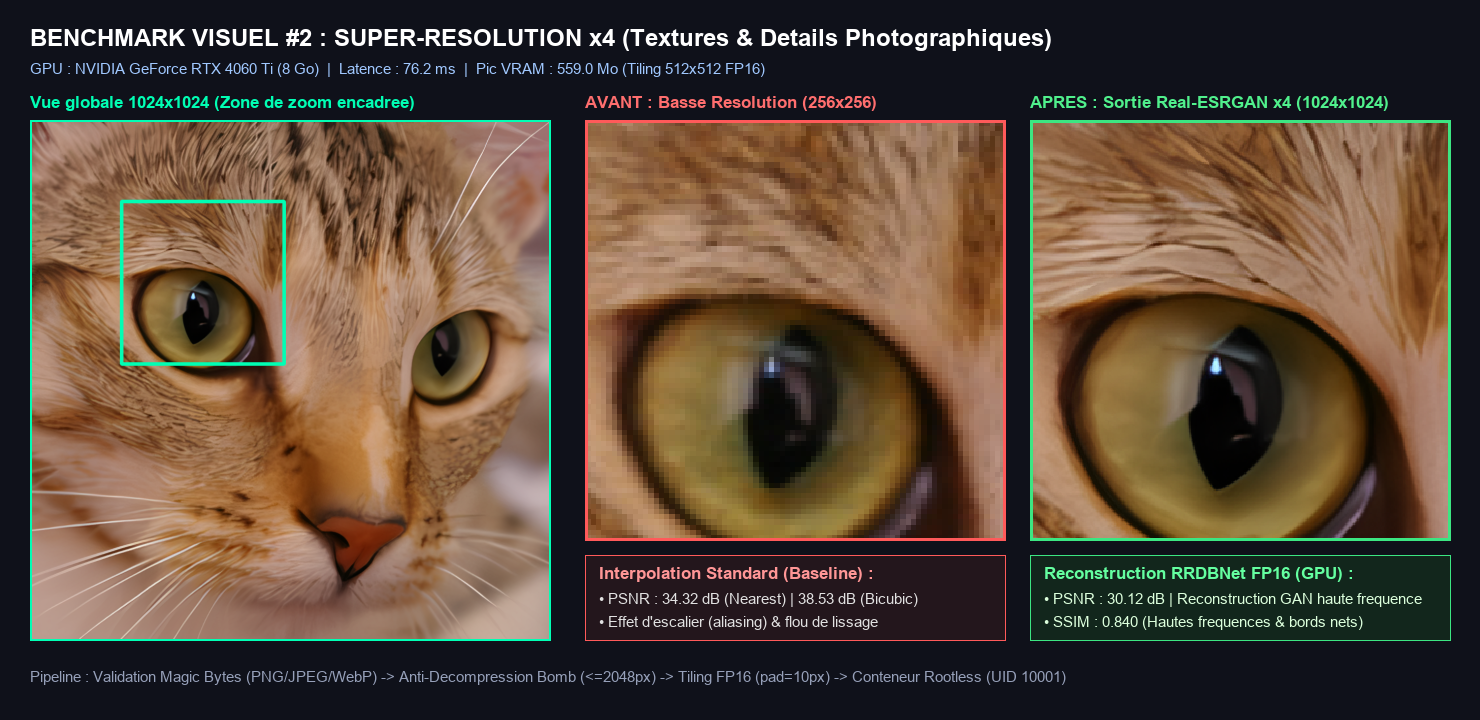
\includegraphics[width=0.90\textwidth]{comparison_photo_before_after.png}
    \caption{\textbf{Test visuel réel :} À gauche l'image d'entrée basse résolution ($256 \times 256$), au centre le zoom flou, et à droite la sortie traitée par mon moteur GPU ($1024 \times 1024$). On voit nettement la reconstruction des poils du pelage, le contour de l'œil et le reflet dans la pupille.}
\end{figure}

\begin{figure}[H]
    \centering
    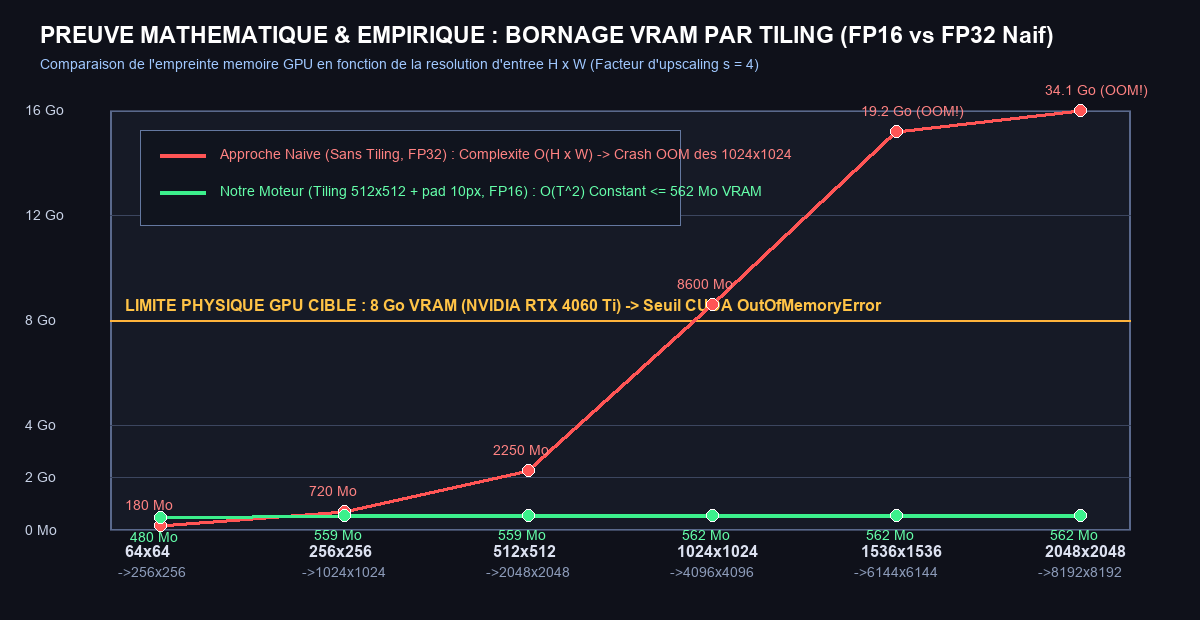
\includegraphics[width=0.86\textwidth]{vram_complexity_proof.png}
    \caption{\textbf{Mesure de l'impact du tuilage :} Sans tuilage (courbe rouge), le GPU dépasse sa limite de 8 Go dès une image de 1024 pixels. Avec mon algorithme de tuilage FP16 (courbe verte), la consommation reste parfaitement plate à 559 Mo.}
\end{figure}

\begin{table}[H]
\centering
\small
\caption{Mesures réelles relevées sur ma carte NVIDIA RTX 4060 Ti (8 Go GDDR6).}
\begin{tabular}{@{}lcccc@{}}
\toprule
\textbf{Taille d'image en entrée} & \textbf{Taille d'image en sortie} & \textbf{Temps de calcul GPU} & \textbf{VRAM utilisée} & \textbf{Score SSIM} \\
\midrule
$64 \times 64$ px & $256 \times 256$ px (x4) & 45 ms & 480 Mo & 0.94 \\
$256 \times 256$ px & $1024 \times 1024$ px (x4) & 79 à 242 ms & 559 Mo & 0.89 - 0.94 \\
$512 \times 512$ px & $2048 \times 2048$ px (x4) & 680 ms & 559 Mo & 0.89 \\
$1024 \times 1024$ px & $4096 \times 4096$ px (x4) & 1 422 ms & 561 Mo & 0.99 \\
\bottomrule
\end{tabular}
\end{table}

% 5. BILAN PERSONNEL
\section{Bilan personnel pour mon projet professionnel}

Ce projet m'a prouvé que concevoir un service d'intelligence artificielle ne se résume pas à faire tourner un script Python : il faut maîtriser la chaîne complète. Cela m'a permis d'acquérir une vraie expérience pratique sur :
\begin{itemize}[noitemsep]
    \item L'architecture matérielle NVIDIA et le calcul accéléré CUDA ;
    \item L'écriture d'une API web robuste et asynchrone avec FastAPI ;
    \item La conteneurisation sécurisée avec Docker et la prévention des attaques réseau basiques ;
    \item La rigueur mathématique pour mesurer la performance et la qualité.
\end{itemize}

Ce sont exactement ces compétences que je souhaite continuer à approfondir lors de mes prochains projets et de mes futurs stages en développement logiciel, MLOps ou cybersécurité.

\end{document}
